\subsection{L’épuisement des ressources}

Pour suivre la demande croissante liée à l'\op, les industriels sont forcés d'exploiter de plus en plus les mines, puits de pétroles et autres moyens d'extraction des matières premières.

\bigbreak Elles sont définies par le dictionnaire Larousse comme étant un "matériau d'origine naturelle faisant l'objet d'une transformation et d'une utilisation économique" \cite{LarousseMatiere1eres}. Celles-ci sont nombreuses et utilisées dans de nombreux secteurs à travers le monde. On peut parler de l'eau, du sable, du caoutchouc mais les ressources les plus recherchées sont principalement le pétroles et les métaux, et ce depuis maintenant quelques décennies. L'EIA (Energy Information Administration), l'administration d'information de l'énergie américaine estime que le monde a consommé plus de 30 Milliards de barils de pétrole en 2013, contre environ 25 Milliards en 1993 \cite{EAI}. D'après le site \textit{planetoscope}, 4,3 millions de tonnes de cuivre ont été produites en 2011 \cite{planetoscopeOrCuivre}, mais la demande reste inférieure à l'offre, provoquant l'augmentation des prix du cuivre. La même chose est valable pour l'or, métal le plus recherché, car plus rare. On estime sa production à 2 700 tonnes en 2012 alors que la demande est de 4 800 tonnes, c'est-à-dire qu'on a besoin de plus de 170\% de la production mondiale. On a donc une demande particulièrement centrée sur le pétrole et les métaux.


\subsubsection{L'extraction des métaux : }

Cependant désormais s'ajoutent aux classiques Cuivre, Aluminium, Fer, Nickel, Zinc, Plomb et Étain les nouvelles venues, les Terres Rares. Celles-ci, un groupe composés de 17 éléments, sont principalement utilisées par les industries de hautes technologies. Grâce à elles, on peut fabriquer des colorants, des composants de batteries ou des aimants plus puissants servant dans les alternateurs afin de produire davantage d’électricité. Elles sont donc un besoin important des industriels et sont devenues une ressource recherchée par de nombreux pays à travers le monde. L'Europe a en effet classé dans un rapport publié en 2010 \cite{RapportEuropeenTerresRares} certaines matières premières comme critiques. On y retrouve par exemple l'Antimoine, le Cobalt et toutes les terres rares, tous considérés comme stratégiques.

Les problèmes commencent à se poser ensuite, puisqu'il faut bien entendu récupérer ces matières premières. Certaines sont faciles à extraire. Le sable doit simplement être déplacé, l'eau a "juste" à être pompée, le bois à être coupé. Cependant il y en a qui sont particulièrement contraignantes. L'aluminium, par exemple, doit d'abord être extrait du sol sous forme de bauxite, puis traité pour obtenir le produit fini. Ce sont donc ces ressources qui posent problème pour l'écologie.

En effet, sous prétexte d'approvisionner le marché mondial certains n'hésitent pas à mettre en péril la santé de l'écosystème environnant. L'extraction des minerais du sol se fait généralement dans les mines avec des conditions parfois effroyables pour les travailleurs. La bauxite est ainsi traitée avec de la soude, puis nécessite de grandes quantités d’électricité, qu'il va falloir produire. Le minerai de Zinc est traité plusieurs fois avant d'obtenir réellement du Zinc. Certaines de ces opérations sont dangereuses pour l'environnement.

\bigbreak
Pour reprendre l'exemple des terres rares, la Chine est devenue le principal exportateur avec 95\% de la production mondiale en possédant seulement 37\% des ressources minières \cite{MongolieChine}. Cela est dû à la pollution qu'implique l'extraction et le raffinage du minerai. Le coût environnemental est tel que des pays comme les États-Unis ou l'Australie ont stoppé leurs activités. Des produits chimiques, des poussières et même de la radioactivité sont évacués durant le processus de traitement. Aux États-Unis, l'entreprise \textit{Molycorp} a ainsi été forcée à la fermeture en 2002 suite à des normes environnementales plus drastiques.

Ainsi en Chine, les mineurs ne possèdent qu'un simple masque leur protégeant une partie du visage. Les autorités semblent fermer les yeux sur les produits déversés dans des lacs. Les populations locales souffrent de problèmes respiratoires et de cancer. L'avantage est que le manque de protection environnementale diminue les coûts de production. Si les états du nord devaient produire des terres rares avec les normes en vigueur, le prix serait bien plus important. On revient donc à l'une des problématiques de l'\op : acheter son produit plus cher pour la santé de l'environnement, ou préférer un prix moins élevé, avec les conséquences que cela induit.


\bigbreak Cette sur-utilisation risque de conduire à terme à une diminution de l'approvisionnement, voire un manque de certaines matières premières.


L'avenir des métaux est également inquiétant. On les retrouve dans quasiment toutes les activités industrielles, du bâtiment à l’électronique en passant par la construction automobile. Le livre "Quel futur pour les métaux ?" \cite{LivreFuturMetaux} présente ainsi un diagramme des réserves supposées de métaux et de la part de marché des trois premiers pays producteurs.

\begin{figure}[h]
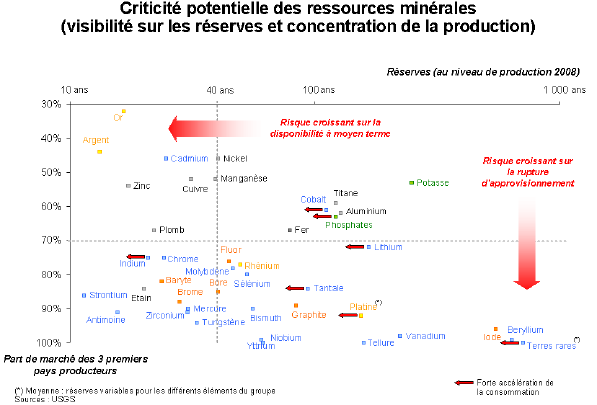
\includegraphics[scale=0.75]{Rsc/risquemetaux.png}
\caption{Schéma présentant la criticité des principaux métaux utilisés}
\label{CriticiteMetaux}%attention, à placer après le caption, sinon référencera la section
\end{figure}

\bigbreak La figure \ref{CriticiteMetaux} présente les réserves et la part de marché des 3 premiers pays producteurs par ressource minérale. On remarque premièrement que le Plomb et le Cuivre sont considérés comme manquant d'ici 40 ans et même 20 pour l'Or, le Zinc et l'Argent. Parallèlement, certaines ressources sont présentes en grandes quantités mais la rupture d'approvisionnement est importante, celle-ci étant liée au nombre de pays producteurs.


\subsubsection{Le cas du pétrole : }

En ce qui concerne le pétrole, utilisé pour les transports mais également pour la production de matières plastiques en tout genre, les avis sont partagés. Les plus alarmistes pensent que le pic d'utilisation est atteint et que désormais, on devra économiser. Pour d'autres, on ne manquera pas de pétrole, puisque de grandes réserves existent dans le sol, sous forme de sable bitumineux ou de gaz de schistes. Ceux-ci pourraient être extraits, mais à l'aide de techniques considérées souvent comme polluantes. La France a ainsi stoppé les industriels à ce niveau. De plus, l'énergie apportée aux machines pour l'extraction ou la transformation d'un litre de pétrole selon ces techniques dépasse parfois l’énergie produite par ce même litre de pétrole. On a ainsi une perte énergétique peu intéressante et surtout polluante.

Il en va de même pour le bioéthanol, qui subit une controverse sur sa réelle utilité. Les écologistes arguent que la production des matières végétales, qui est parfois considérée comme polluante (pesticides, ...) utilise également plus de pétrole pour les tracteurs, le transport, ... , que ce qui est gagné en le remplaçant par de l’éthanol. Le pétrole est donc aléatoire pour certains, et risque peut-être d'être plus cher dans les années à venir.


\subsubsection{L'impact écologique : } 

Quelques organisations et états ont commencé à chercher des indicateurs de l'impact humain sur la planète.

La première est la dette écologique. D'après l'ONG \textit{Footprint Network}, la population vit à crédit depuis le 19 août cette année \cite{DateACredit}. Cette date correspond au jour où toutes les ressources consommées durant l'année sont trop importantes pour pouvoir être renouvelées. On vivrait ainsi "à crédit" à partir de cette date, portant une dette écologique. Le jour de ce dépassement était le 22 Septembre en 2003 et le 21 octobre en 1993. On remarque que cela arrive de plus en plus tôt au fil des ans et on peut aisément craindre que cette tendance se poursuive.

L'empreinte écologique est un autre indicateur. Elle correspond à la pression exercée par l'homme sur la nature. On calcule le nombre d'hectares globaux (hag), c'est-à-dire une surface, dont une population a besoin pour générer ses ressources, puis les absorber. La valeur critique est de 1.8 hag. Si tout le monde avait cette empreinte, on utiliserait 100\% de notre planète. Pour un Français moyen, celle-ci est de 4.6 hag, ce qui signifie qu'il faudrait avoir 2.5 planètes pour absorber les déchets si toute la population mondiale était composée de Français. Les Américains ont besoin du double (9 hag).

\bigbreak
Les ressources naturelles sont donc particulièrement demandées et certaines risquent de manquer dans les années à venir. De plus leur extraction est parfois dangereuse et surtout polluante. L'\op est particulièrement liée à ce phénomène, puisque la fabrication de masse inhérente au modèle implique une forte demande toujours renouvelée. On peut ainsi craindre une pénurie de certaines ressources particulièrement importante, tels que l'eau ou le pétrole, pour les générations à venir.

\medbreak
Cependant, l'extraction des matières premières n'est pas le seul danger pour l'environnement. En effet l'utilisation faite de celles-ci à un effet néfaste pour l'environnement.

%cite{LarousseMatiere1eres}

%cite{sociétéChimiqueDeFranceTerresRares}

%cite{RapportEuropeenTerresRares}

%cite{MongolieChine}

%cite{LivreFuturMetaux}

%cite{DateACredit}
